\documentclass[11pt,fleqn]{article}
\usepackage{../cs188,latexsym,epsf, amsmath,amsfonts,graphicx,url}
\lecture{6}
\def\title{Note \the\lecturenumber}
\begin{document}
\maketitle


\iffalse
\documentclass[11pt,fleqn]{article}
\usepackage{latexsym,epsf,amsmath,amsfonts,graphicx,url}

\title{Note 6}

\newcommand{\F}{\mathbb{F}}
\newcommand{\Z}{\mathbb{Z}}
\newcommand{\Q}{\mathbb{Q}}
\newcommand{\R}{\mathbb{R}}
\newcommand{\C}{\mathbb{C}}

\begin{document}

\maketitle
\fi

\section*{Bayes Nets}
In artificial intelligence, we often want to model the relationships between various nondeterministic events. If the weather predicts a 40\% chance of rain, should I carry my umbrella? How many scoops of ice cream should I get if the more scoops I get, the more likely I am to drop it all? If there was an accident 15 minutes ago on the freeway on my route to Oracle Arena to watch the Warriors' game, should I leave now or in 30 minutes? All of these questions (and innumerable more) can be answered with \textbf{Bayesian networks} (Bayes nets for short), graphical models that capture the conditional independence relationships between variables we want to represent and when done correctly can allow us to make good predictive inferences about various questions we wish to answer. Let's get started by discussing how Bayes' nets are constructed. <DONT LIKE THIS MAKE IT BETTER>

\section*{Representation}

In previous sections of this class, we modeled the world as existing in a specific state that is always known. For the next several weeks, we will instead use a new model where each possible state for the universe has its own probability. For example, we might build a weather model, where the state consists of the season, temperature and weather. Our model might say that $P(winter, 35 fahrenheit, cloudy) = 0.00023$.

In such a model, the state of the universe is simply a \textbf{joint distribution}, i.e. a table of probabilities which captures the likelihood of multiple events [check] occuring simultaneously. 

Given such a model, we can trivially perform any kind of probability inference using the intuitive \textbf{Inference by Enumeration} technique discussed during the probability lecture.

Naturally, representing an entire joint distribution in the memory of a computer is not very scalable - if each of $n$ variable we wish to represent can take on $d$ possible values (it has a \textbf{domain} of size $d$), then our joint distribution table will have $d^n$ entries! 

Bayes nets avoid this issue by choosing to store information in small, local probability tables along with a \textbf{directed acyclic graph} which captures the relationships between variables. With this efficient storage, we can recompute any desired probabilities on demand by running \textbf{probabilistic inference} on the local probability distributions. 

Specifically, each node in the graph represents a single random variable. Arrows in the graph represent conditional independent relationships. A node is conditionally independent of its ancestors given all of its parents. Thus, if we have a node representing variable Q, we store $P(Q | X_1, X_2, ..., X_N)$, where $X_1, ..., X_N$ are the parents of Q.

As an example of a Bayes Net, consider a model where we have five binary random variables described below:

\begin{itemize}
\item B: Burglary occurs.
\item A: Alarm goes off.
\item E: Earthquake occurs.
\item J: John calls.
\item M: Mary calls.
\end{itemize}

Assume the alarm can go off if either a burglary or an earthquake occurs, and that Mary and John will call if they hear the alarm. In this case, we can represent the natural conditional independences with the graph shown below.

\begin{center}	
	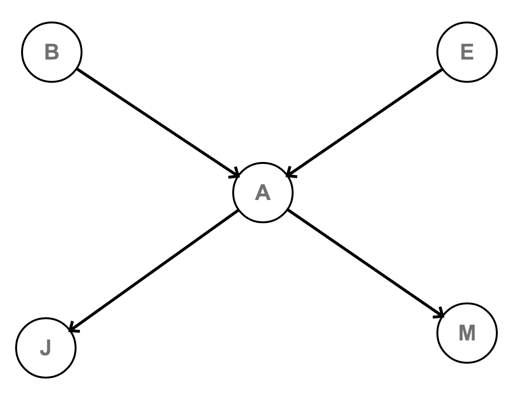
\includegraphics[width=10cm]{img/alarm_model}
\end{center}

Models capture a way the world works - they are always a simplification - key
all models are wrong, but some will still be useful for solving real problems in the real world. They may may not account for every variable or even every interaction between variables.

\section*{Representation}

BAYES NETS -- the joint distribution is usually too hard to represent in many cases - you have a whole bunch of variables with many domains $d^N$ scales very quickly
the solution is to have a more structured representation in the form of bayes nets to decompose a large joint distribution into simple local distributions which can then be pieced together to build up any other more global distributions that are desired

NOTATION: nodes (variables), arcs (interactions between variables -- formally encode conditional independence)
bayes nets are directed acyclic graphs
have a conditional distribution for each node X
P(X | a1 a2 ... an) each thing is a key thing conditional based on parents

how to convert from bayes to full join probability - product P(xi | parents(xi)) <-- show validity of this using chain rule


causality??

\section*{Inference}

INFERENCE

BY ENUMERATION
Given some evidence, calculate some useful probability you want to know
inference is np-complete, but you can improve its performance usually in a key way
evidence, query, and hidden variables
evidence - things we have observed
query - what we want to predict
hidden - variables in the bayes net we must get rid of 

VARIABLE ELIMINATION
optimization on inference by enumeration by summing out at intermediary steps rather than just at the end
select hidden variables in some order - join all factors mentioning H then sum out over it
how to select ordering of variables? -- computational complexity very dependent on the largest factor involved

different types of factors


\subsection*{D-Separation}
One very common question about Bayes' nets that comes up very frequently both in this class and in application is that of the conditional independence between its variables. This is something that's often incredibly unintuitive to reason through

\section*{Sampling}



\end{document}